\documentclass[12pt]{article}

\usepackage{geometry}
\usepackage[utf8]{inputenc}
\usepackage[T2A]{fontenc}
\usepackage[russian]{babel}
\usepackage{graphicx}
\usepackage{caption}
\usepackage{amssymb, gensymb, amsmath}
\usepackage{mathrsfs}
\usepackage{array, colortbl}
\usepackage{multicol}

\title{{\bf Лабораторная работа 1.\, 2. \\ Исследование эффекта Комптона}}
\author{Лось Денис (группа 618)}
\date{26 сентября 2018}

\begin{document}

\maketitle

\paragraph{Цель работы: } исследовать энергетический спектра $\gamma$-квантов, рассеянных на графите, определить энергию рассеянных $\gamma$-квантов в зависимости от угла рассеяния, а также энергию покоя частиц, на которых происходит комптоновское рассеяние, исследовать эффект Комптона.

\section*{Теоритическое введение}
\par
	Рассеяние $\gamma$-лучей в веществе относится к числу явлений, в которых особенно ясно проявляется двойственная природа излучения. Волновая теория, хорошо объясняющая рассеяние длинноволонового излучения испытывает трудности при описании рассеяния рентгеновских и $\gamma$-лучей. Эта теория, в частности, не может объяснить, почему в составе рассеянного излучения, измеренного Комптоном, кроме исходной волны с частотой $\omega_0$ появляется дополнительная длинноволновая компоненента, отсутствующая в спектре первичного излучения.
\par
	Появление этой компоненты легко объяснимо, если считать, что $\gamma$-излучение представляет собой поток квантов(фотонов), имеющих энергию $\hslash \omega$ и импульс $p = \hslash \omega / c$. Эффект Комптона --- увеличение длины волны рассеянного излучения по сравнению с падающим --- интерпретируюется как результат упрогого соударения двух частиц: $\gamma$-кванта(фотона) и свободного электрона.
\par
	Рассмотрим элементарную теорию эффекта Комптона. Пусть электрон до соударения покоился (его энергия равна энергии покоя $mc^2$), а $\gamma$-квант имел начальную энергию $\hslash \omega_0$ и импульс $\hslash \omega_0 / c$. После соударения электрон приобретает энергию $\gamma mc^2$ и импульс $\gamma m v$, где $\gamma = (1 - \beta^2)^{-1/2}$, $\beta = v / c$, а $\gamma$-квант рассеивается на некоторый угол $\theta$ по отношению к первоначальному направлению движения. Энергия и импульс кванта становятся соотвественно равными $\hslash \omega_1$ и $\hslash \omega_1 / c$.
\par
	Законы сохранения энергии и импульса:
\begin{align*}
	mc^2 + \hslash \omega_0 = \gamma mc^2 + \hslash \omega_1 \\
	\frac{\hslash \omega_0}{c} = \gamma mv \cos \varphi + \frac{\hslash \omega_1}{c} \cos \theta \\
	\gamma m v \sin \varphi = \frac{\hslash \omega_1}{c} \sin \theta
\end{align*}
\par
	Решив совместно эти уравнения и сделав переход от частот $\omega_0$ и $\omega_1$ к длинам  волн $\lambda_0$ и $\lambda_1$, получим, что изменение длины волны рассеянного излучения равно
\begin{equation}
	\Delta \lambda = \lambda_1 - \lambda_0 = \frac{h}{mc}\left(1 - \cos \theta \right) = \Lambda_\text{к} \left(1 - \cos \theta \right), \label{main} 
\end{equation}
где $\lambda_0$ и $\lambda_1$ --- длины волн $\gamma$-кванта до и после рассеяния, а величина
\[
	\Lambda_\text{к} = \frac{h}{mc} = 2.42 \cdot 10^{-10} \, \text{см}
\]
называется комптоновской длиной волны.
\par
	Преобразованное выражение (\ref{main}) от длин волн к энергии $\gamma$-квантов
\begin{equation}
	\frac{1}{\varepsilon(\theta)} - \frac{1}{\varepsilon_0} = 1 - \cos \theta. \label{main2}
\end{equation}
\par
	Здесь $\varepsilon_0 = E_0 / (mc^2)$ --- выраженная в единицах $mc^2$ энергия $\gamma$-квантов, падающих на рассеиватель, $\varepsilon(\theta)$ --- выраженная в тех же единицах энергия квантов, испытавших комптновоское рассеяние на угол $\theta$, $m$ --- масса электрона.
\par
	Заменим в формуле (\ref{main2}) энергию квантов, испытавших комптоновское рассеяние на угол $\theta$, номеров канала $N(\theta)$, соотвествующего вершине фотопика при указанном угле $\theta$. Обозначая буквой $A$ неизвестный коэффициент пропорциональности между $\varepsilon(\theta)$ и $N(\theta)$, найдём
\begin{equation}
	\frac{1}{N(\theta)} - \frac{1}{N(0)} = A \left(1 - \cos \theta \right)
\end{equation}
\par
	Для энергии покоя частицы имеем
\begin{equation}
	mc^2 = E(0) \, \frac{E(90)}{E(0) - E(90)} = E_\gamma \, \frac{N(90)}{N(0) - N(90)}.
\end{equation}

\section*{Ход работы и результаты исследования}
\par
	Снимем зависимость номера канала $N(\theta)$ от угла $\theta$ и построим график зависимости $1 / N(\theta)$ от $1 - \cos \theta$, принимая во внимание ошибку измерений. По полученному графику проведём наилучшую прямую и определим энергию покоя частицы.
\newpage
\begin{table}[h!]
	\centering
	\begin{tabular}{|c|c|c|c}
	\hline
		Угол отклонения $\theta \degree$ & Номер канала $N(\theta)$ & $1 / N(\theta) \cdot 10^{-3}$ \\
	\hline
		0&	964	&1.04 \\
	\hline
10	&941& 1.06 \\
\hline
20	&813& 1.23 \\
\hline
30	&765& 1.31 \\
\hline
40	&704&	1.42 \\
\hline
50	&612&	1.63 \\
\hline
60	&533&	1.88 \\
\hline
70	&475&	2.11 \\ 
\hline
80	&430&	2.33 \\	
\hline
90	&384&	2.60 \\
\hline
100	&350&	2.86 \\
\hline
110	&325&	3.08 \\
\hline
120	&295&	3.39 \\
	\hline
	\end{tabular}
\end{table}
\begin{figure}[h!]
	\centering
	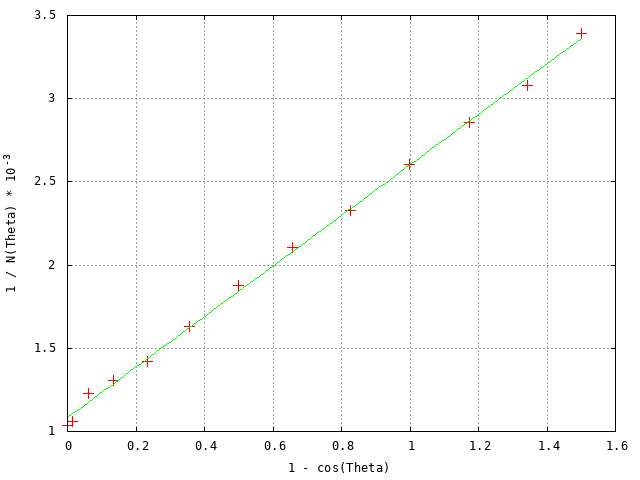
\includegraphics[width = 14cm, height = 9cm]{plot1.png}
	\caption{График зависимости $1 / N(\theta) = f \left(1 - \cos \theta \right)$}	
\end{figure}
\newpage
	Из графика получим, что коэффициент наклона графика $\beta$ и $N(0 \degree)$, а также $N(90 \degree)$ равны
\begin{align*}
	\beta &= \left(15.2 \pm 0.2\right) \cdot 10^{-4} \\
	N(0 \degree) &= \left(924 \pm 13\right) \\
	N(90 \degree) &= \left(383\pm 5\right)
\end{align*}
\par
	Следовательно, найденная энергия покоя электрона равна
\[
	mc^2 = E_\gamma \, \frac{N(90 \degree)}{N(0 \degree) - N(90 \degree)} = \left(469 \pm 14 \right) \, \text{кэВ}
\]
\par
	Полученное значение лежит близко к известной величине $E = 511$ кэВ для энергии покоя электрона, однако значения не находятся в пределах найденной абсолютной погрешности.
\end{document}